Para tener un buen desarrollo y despliegue del proyecto se decidio por utilizar la herramienta \textbf{Docker}, esta herramienta nos permite trabajar con contenedores que empaquetan la aplicación desarrollada, los distintos archivos de codigo, conexiones a bases de datos, entornos virtuales (.env), archivos de configuración, dependencias, etc \cite{docker-docs}. Estos contenedores de docker se almacenan en repositorios de contenedores (parecido a Github), permitiendo ser portable entre distintos desarrolladores a través de una imagen basada en linux, esta imagen contiene todos los archivos relevantes de la aplicación y es ejecutada en un contenedor de docker. Los contenedores son varias de estas imagenes juntas, por lo general, la primera capa corresponde a una distribución de linux. Los contenedores virtualizan la aplicación y utilizan el kernel del sistema operativo anfitrión, reduciendo el tamaño y tiempo de ejecución de la aplicación en gran manera.

Para empaquetar la aplicación en un contenedor de docker se siguieron los siguientes pasos:

\begin{itemize}
    \item Primero creamos un archivo \textbf{Dockerfile}, el cual sera usado para crear la imagen de la aplicación, en este archivo especificamos la imagen de la versión de Python a utilizar, en este caso la 3.9 para permitir el correcto funcionamiento de las otras dependencias, copiamos el archivo que contiene los requerimientos de la aplicación y luego se ejecuta una linea que instala estos requerimientos, para contener todos los archivos de la aplicación, se copia la ruta de la carpeta y todo su contenido. Se espeficia el puerto al cual docker enlazara el contenedor creado y se escriben los comandos necesarios para ejecutar la aplicación. Todos estos comandos serán ejecutados cuando se cree un nuevo contenedor.
    \begin{figure}[H]
        \begin{minipage}[t]{0.9\textwidth}
            \caption{Código archivo Dockerfile}
            \label{Docker_creation}        
        \end{minipage}
    
        \vspace{10pt}
    
        \begin{minipage}[b]{1\textwidth}
            \centering
            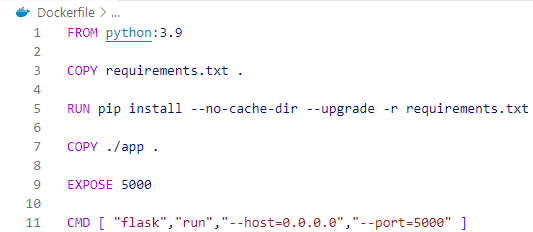
\includegraphics[width=\textwidth]{img/dockerfile.png}        
        \end{minipage}
    
        \begin{minipage}[t]{0.9\textwidth}
            Fuente: Elaboración propia.
        \end{minipage}
    \end{figure}

    \item Como segundo paso, se crea un archivo \textbf{.dockerignore} en el cual se especifican todas las carpetas y archivos que no deben de ser considerados en la creación de la imagen de docker.

    \item El ultimo paso en la dockerización de la aplicación, es la creación de un archivo \textbf{docker-compose.yml} el cual puede contener y gestionar varios servicios de docker. En este caso solo contendra un servicio, este servicio corresponde a la aplicación que se busca contener, se especifican los nombres del contenedor e imagen a crear, el puerto a ocupar y como se creara el contenedor de docker, indicando el contexto y nombre del archivo para crear la imagen, en este caso Dockerfile.

    \begin{figure}[H]
        \begin{minipage}[t]{0.9\textwidth}
            \caption{Código archivo docker-compose.yml}
            \label{docker_compose}        
        \end{minipage}
    
        \vspace{10pt}
    
        \begin{minipage}[b]{1\textwidth}
            \centering
            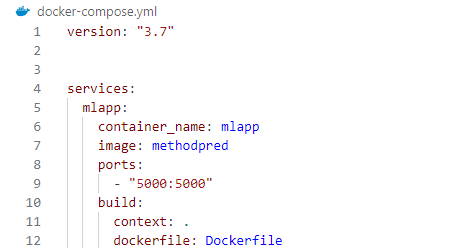
\includegraphics[width=\textwidth]{img/docker-compose.png}        
        \end{minipage}
    
        \begin{minipage}[t]{0.9\textwidth}
            Fuente: Elaboración propia.
        \end{minipage}
    \end{figure}

\end{itemize}

Con los pasos anteriormente mencionados realizados, se puede proceder a ejecutar el comando \textquotedblleft docker-compose up $--$build\textquotedblright , este comando procedera a crear y ejecutar un contenedor basado en la imagen especificada. Con esto se asegura un despliegue de la aplicación sin problemas de rendimiento, tamaño de modulos o discrepancias en las versiones de los módulos.